\chapter{Introduction}
\label{ch:introduction}
\begin{figure}[tb]
  \centering
  \vspace{10pt}
  % 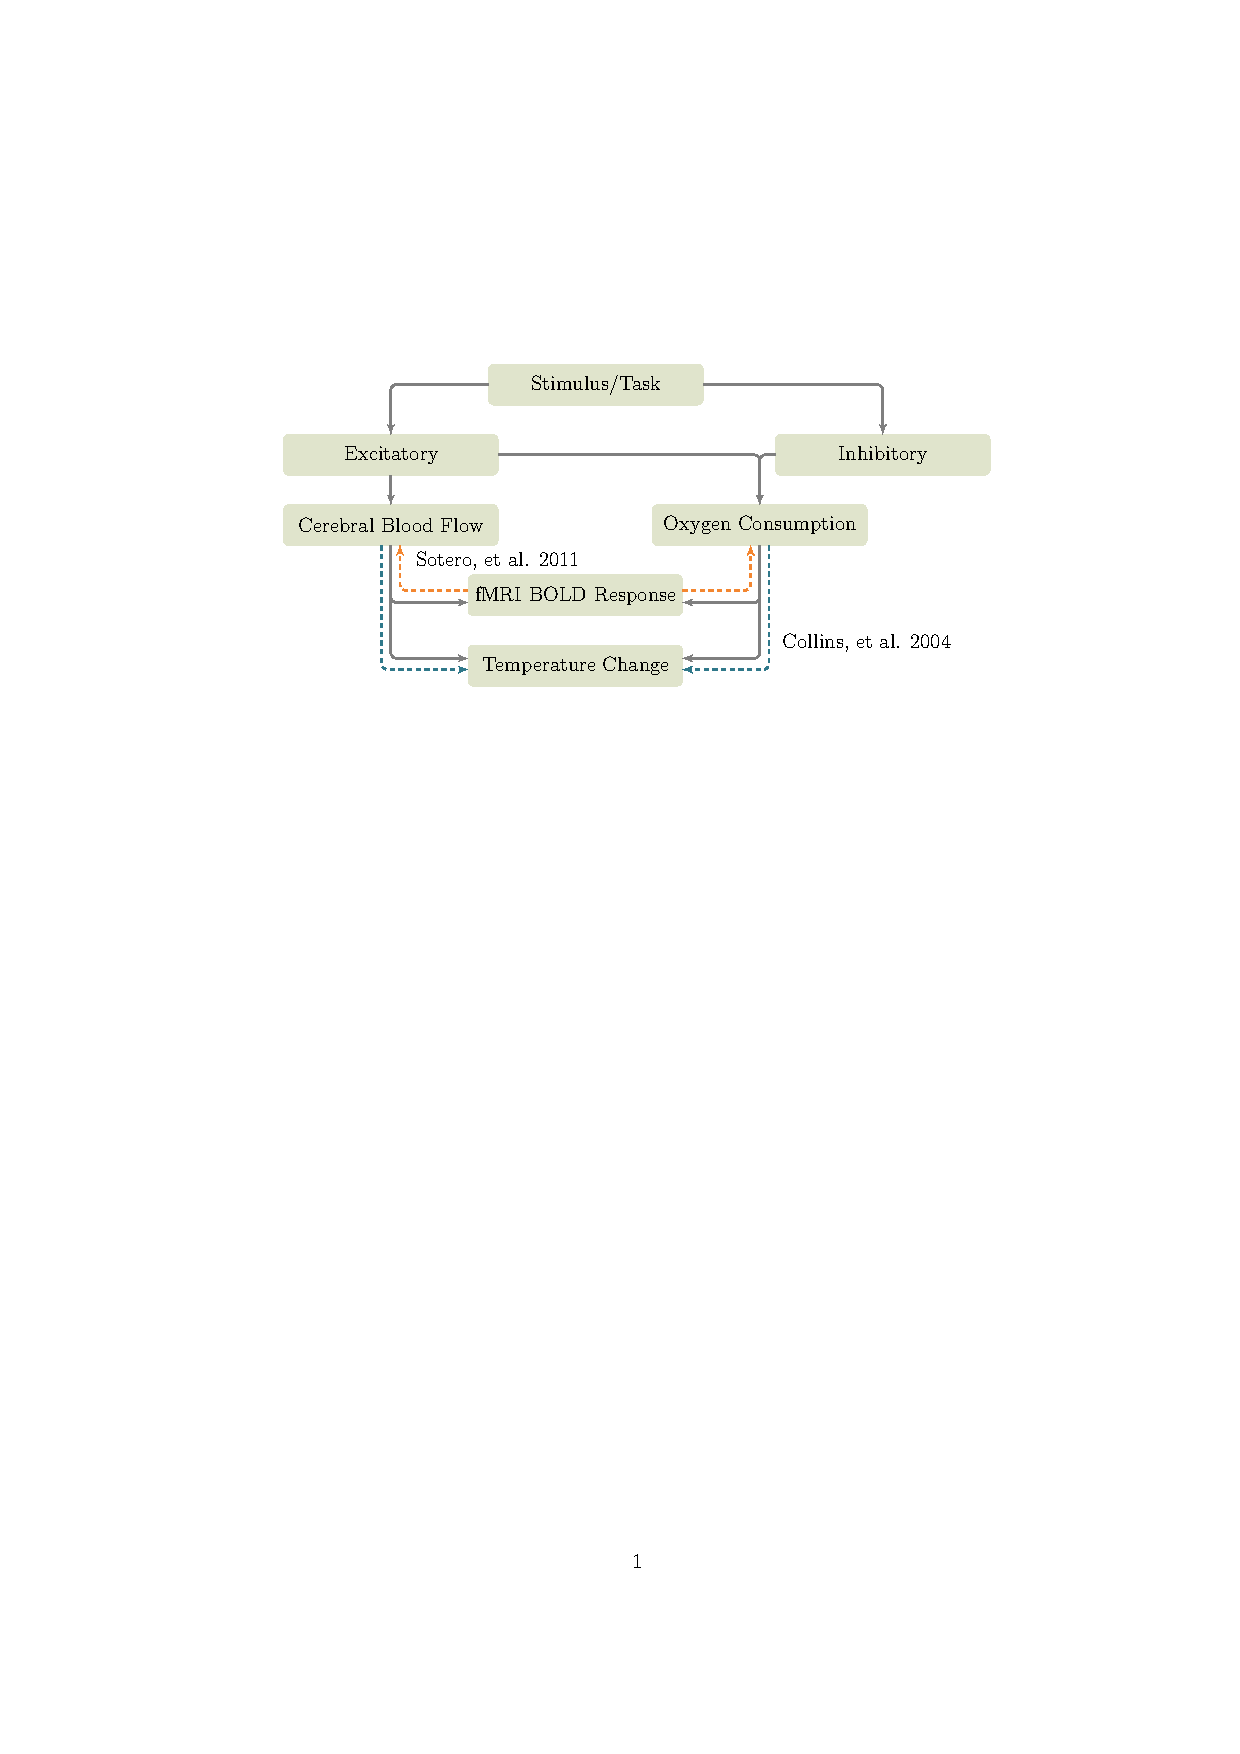
\includegraphics{flowchart}
  \tikzstyle{block} = [draw=none, fill=beachstorm]
\tikzstyle{line} = [draw, very thick, color=black!50, -stealth']
\tikzstyle{sotero} = [draw, very thick, dashed, color=goldfish, -stealth']
\tikzstyle{collins} = [draw, very thick, dashed, color=aoi, -stealth']
\tikzstyle{citation} = [draw=none, fill=white, minimum height=0.5cm, anchor=north, text width=6.5cm]

\begin{tikzpicture}[node distance=0.7cm, rectangle, text width=4.5cm, text badly centered, rounded corners, minimum height=1cm, anchor=north]
  \node[block](stimulus){Stimulus/Task};
  
  \node[block, below=of stimulus, xshift=-5cm](excitatory){Excitatory Neuronal Activity};
  \node[block, below=of stimulus, xshift= 7cm](inhibitory){Inhibitory Neuronal Activity};
  
  \node[block, below=of excitatory](cbf){Increase in Cerebral Blood Flow (CBF)};
  \node[block, below=of inhibitory, xshift=-3cm](o2){Change in Oxygen Consumption (CMRO$_2$)};
  
  \node[block, below=of cbf, xshift=4.5cm, yshift=-0.5cm](bold){fMRI BOLD Response};
  \node[block, below=of bold](temp){Temperature Change};
  
  \node[citation](sotero1) at (-1.6, -5) {\citet{sotero2011}};
  % \node[citation](sotero1) at (2, -4.5) {Sotero, et. al. 2011};
  % \node[citation](sotero1) at (-4.5, -7.5) {Collins, et. al. 2011};
  \node[citation](sotero1) at (6, -6.5) {\citet{collins}};
  
  \path[line](stimulus.west) -| (excitatory.north);
  \path[line](stimulus.east) -| (inhibitory.north);
  \path[line](excitatory.south) -- (cbf.north);
  \path[line](excitatory.east) -| (o2.north);
  \path[line](inhibitory.west) -| (o2.north);
  
  \path[line](cbf.south) |- ([yshift=-5pt] bold.west);
  \path[line](cbf.south) |- ([yshift= 5pt] temp.west);
  \path[line](o2.south)  |- ([yshift=-5pt] bold.east);
  \path[line](o2.south)  |- ([yshift= 5pt] temp.east);
  
  \path[sotero]([yshift= 5pt] bold) -| ([xshift= 20pt] cbf);
  \path[sotero]([yshift= 5pt] bold) -| ([xshift=-20pt] o2);
  \path[collins]([xshift=-45pt] cbf) |- ([yshift=-5pt] temp);
  \path[collins]([xshift=45pt] o2)  |- ([yshift= -5pt] temp);
\end{tikzpicture}
  \caption[Generation of the fMRI BOLD response and a corresponding temperature change]{\label{fig:flowchart} Generation of the fMRI BOLD response from changes in neuronal activity.  Black arrows indicate a causal relationship while colored dashed-arrows indicate existing models for the relationship.  The orange line ($\color{goldfish}\bullet$) shows the model proposed by~\citet{sotero2011} to calculate cerebral blood flow and metabolism and the blue line ($\color{aoi}\bullet$) shows how the model proposed by~\citet{collins} is used to calculate temperature.  Modified after~\citet{sotero2007}.}
\end{figure}

Since its invention in the 1950's~\citep{carr1954} and later development in the 1970's~\citep{lauterbur1973}, {M}agnetic {R}esonance {I}maging ({MRI}) has allowed physicians and scientists a detailed view within the human body.  Beginning in the 1990's, it was realized that changes in the local metabolic state affect the local magnetic resonance and provide an indication of brain activity~\citep{ogawa1990,kwong1992}.  This is possible because hemoglobin is diamagnetic in an oxygenated state and paramagnetic when deoxygenated.  Thus as the local concentration of deoxyhemoglobin changes, the local magnetic susceptibility is also altered.  

By combining this effect with a discovery made earlier in 1986 ~\citep{fox1986}, MRI becomes a powerful tool for measuring brain activity.  \Citet{fox1986} found that with an increase in neuronal activity came an increase in local cerebral blood flow (CBF) that exceeded the increase in cerebral metabolic rate of oxygen (CMRO$_2$).  The change in local tissue oxygenation created by uncoupled changes in CBF and CMRO$_2$ is referred to as the blood oxygen dependent~(BOLD) response~\citep{kwong1992}.  A schematic of the model for generation of the fMRI BOLD response is provided in~\cref{fig:flowchart}.

A stimulus within a region of the brain induces either an excitatory or inhibitory (or a combination) neuronal response.  An increase in excitatory neuronal activity triggers an increase in CBF which overcompensates for the increase in CMRO$_2$~\citep{fox1986}.  Conversely, an increase in inhibitory neuronal activity does not induce a change in CBF.  Increasing CMRO$_2$ increases the concentration of deoxyhemoglobin (deoxyHb) while increasing CBF delivers more blood to the tissue thereby increasing the concentration of oxyhemoglobin (oxyHb) and increasing local tissue oxygenation.  The change in blood oxygenation is detected by the fMRI as the BOLD response~\citep{kwong1992}.

Along with changes in the BOLD response, changes in CBF and CMRO$_2$ also affect the local tissue temperature. As glucose is metabolized, heat is released that is primarily dissipated by convection to blood.  Thus, a change in rate of blood flow will affect how quickly heat can be dissipated (or delivered as we'll explore in~\cref{sec:results}).  Since both BOLD and temperature are dependent on CBF and CMRO$_2$, it is possible to use the BOLD data collected to calculate the temperature change. As will be further discussed in~\cref{sec:theoreticalresults}, the resulting temperature change cannot be easily characterized for the entire brain because it's behavior is spatially dependent.

Experimental measurements of activity-induced brain temperature changes are mixed in whether an increase in brain activity increases or decreases local tissue temperature~\citep{mcelligott,kiyatkin,zeschke,george,tachibana}. Current temperature models predict that an increase in activity will result in a decrease in temperature~\citep{sotero2011,yablonskiy,trubel}.  This is generally the prediction because these models generalize the resting-state conditions of the voxel (ignoring spatial dependence) which puts the blood temperature below the resting state tissue temperature.  An increase in blood flow then acts as a coolant for the tissue and lowers the temperature (more on this in~\cref{sec:tempmodelintro}).

I will explore a model which calculates temperature using the fMRI BOLD response for the entire brain, thereby accounting for spatial dependencies.  Additionally, in~\cref{ch:detectors} I'll explore optical measurement techniques including functional near-infrared spectroscopy (fNIRS) and the use of thermal imaging cameras to measure activity-induced brain temperature changes.